\chapter{栈、队列和数组}\label{DS03}

\par\medskip\noindent\textbf{章节脉络}\par\smallskip
\begin{wideblock}\centering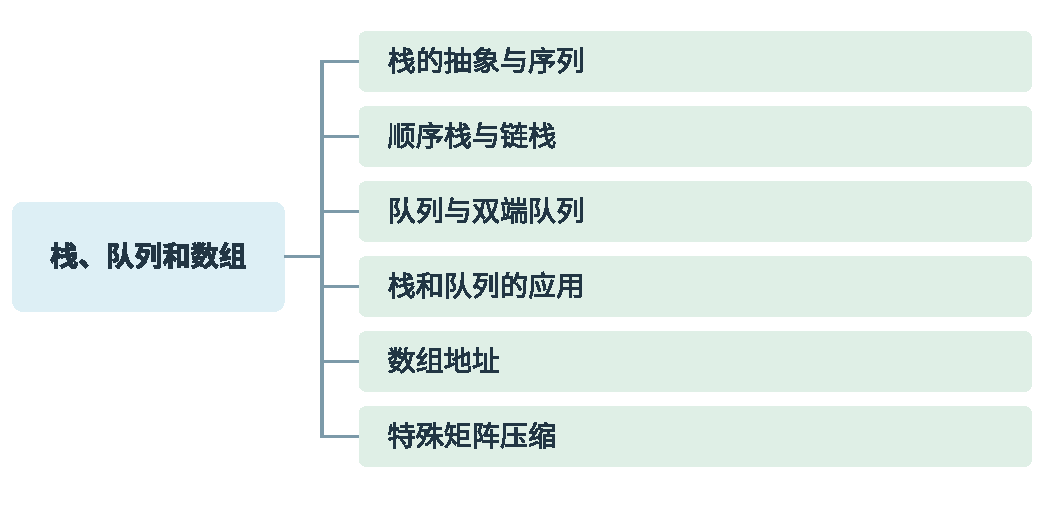
\includegraphics[width=\linewidth,height=92mm,keepaspectratio]{figures/overview.pdf}\end{wideblock}\par\medskip

栈与队列都保存线性序列，差别在于允许从哪一端加入和取出。判断一个操作序列是否合法，必须保留操作过程中的状态；只检查输入、输出是否含有相同元素，不能排除违反栈顶或队头约束的情况。

\section{栈的后进先出与合法序列}\label{DS03-01}

\textbf{栈}只允许在同一端插入和删除，这一端称为栈顶，另一端称为栈底。入栈称 \texttt{push}，出栈称 \texttt{pop}。栈为空时不能出栈；固定容量栈满时不能继续入栈。若中途不出栈，一批元素的出栈次序是入栈次序的逆序；若允许交替入栈和出栈，输出就可能有多种。

检验给定输出的方法是按目标逐个模拟：若当前栈顶不是所需元素，继续把尚未入栈的元素依次压入；一旦所需元素到顶，就弹出。若输入已用尽而栈顶仍不符，输出不合法。这个过程也给出实现该输出所需的最小容量，即模拟中出现的最大栈深。

\subsection{例 3-1　队列不会改变栈的输出次序}\label{DS03-ex1}

\begin{example}[配套例题]

配套例题：栈 \(S\) 和队列 \(Q\) 初始均为空，元素 \texttt{a,\allowbreak{}b,\allowbreak{}c,\allowbreak{}d,\allowbreak{}e,\allowbreak{}f,\allowbreak{}g} 依次入栈 \(S\)。每个元素出栈后立即进入队列 \(Q\)，7个元素出队顺序为 \texttt{b,\allowbreak{}d,\allowbreak{}c,\allowbreak{}f,\allowbreak{}e,\allowbreak{}a,\allowbreak{}g}，则栈容量至少是（　）。

A. 1　B. 2　C. 3　D. 4

\end{example}

\textbf{解析。} 队列保持进入它的先后次序，因此它的输出就是栈的输出。按目标模拟，栈内状态按栈底到栈顶写：

\par\medskip\noindent\begin{minipage}{\linewidth}\fontsize{9.3}{12}\selectfont\begin{tabularx}{\linewidth}{@{}YYY@{}}
\toprule\noalign{}
需要输出 & 必须先执行的入栈 & 弹出后栈内剩余 \\
\midrule\noalign{}


b & a、b & a \\
d & c、d & a、c \\
c & 无 & a \\
f & e、f & a、e \\
e & 无 & a \\
a & 无 & 空 \\
g & g & 空 \\
\bottomrule\end{tabularx}
\end{minipage}\par\medskip

压入 d 或 f 后，栈深达到3；表中过程也说明3个单元足够，答案为 \textbf{C}。不能把队列当作另一处可以随意调整次序的缓冲区。

若只用入栈 \texttt{I}、出栈 \texttt{O} 表示操作，一段从空栈出发并回到空栈的合法序列须满足：两类操作的总数相等，且每个前缀中 \texttt{O} 的个数不超过 \texttt{I}。对 \(n\) 个不同元素，合法出栈序列数为卡特兰数 \(C_n=\frac1{n+1}\binom{2n}{n}\)；这一公式用于计数，不代替具体容量与给定序列的模拟。

输入为 \texttt{a,\allowbreak{}b,\allowbreak{}c,\allowbreak{}d} 时，若输出以 \texttt{c,\allowbreak{}d} 开头，弹出 c 后栈中为 a、b，随后必须压入并弹出 d，剩余只能 b、a，因此仅有 \texttt{c,\allowbreak{}d,\allowbreak{}b,\allowbreak{}a} 一种。若题目指定的是栈的输出而让输入未知，也要反推中间栈顶。例如第3个输入是1，输出从1递增，1弹出时第2个输入压在第1个输入上方；若第1个是2，就要先弹出上面的另一个值才能到2，与``接下来输出2''矛盾，所以第1个不可能是2。

\section{队列与双端队列}\label{DS03-02}

\textbf{队列}只在队尾加入、在队头删除，遵循先进先出。它适合保存等待依次处理的对象，如按发现顺序等待扩展的图顶点。队头与队尾是逻辑角色，不能凭数组下标的大小判断先后：循环队列绕回后，队尾下标可以小于队头下标。

\textbf{双端队列}允许在两端插入和删除。输入受限双端队列只允许一端输入，两端均可输出；输出受限双端队列允许两端输入，只允许一端输出。判断输出时应明确属于哪一种，不能直接套普通队列或普通栈的限制。双端队列能够模拟栈与队列，但这不表示它能按任意次序输出一组顺序输入的元素。

以1、2、3、4依次输入为例，普通栈有14种合法输出。输入受限双端队列有22种，不能输出\texttt{4,\allowbreak{}2,\allowbreak{}1,\allowbreak{}3}和\texttt{4,\allowbreak{}2,\allowbreak{}3,\allowbreak{}1}：先输出4意味着1、2、3已按次序留在队列中，2在中间，下一次无法取出。输出受限双端队列也有22种，不能输出\texttt{4,\allowbreak{}1,\allowbreak{}3,\allowbreak{}2}和\texttt{4,\allowbreak{}2,\allowbreak{}3,\allowbreak{}1}：4第一次输出前，前三个元素只能通过两端依次接入，其剩余次序只能为123、213、312或321，不能为132或231。两种受限队列的非法序列集合并不相同。

\section{顺序栈、共享栈与循环队列}\label{DS03-03}

顺序栈存于 \texttt{A[\allowbreak{}0.\allowbreak{}.\allowbreak{}M-1]\allowbreak{}}。本章令 \texttt{top} 指向当前栈顶，初值 \ensuremath{-}1：空条件 \texttt{top=\allowbreak{}=\allowbreak{}-1}，满条件 \texttt{top=\allowbreak{}=\allowbreak{}M-1}；入栈为 \texttt{A[\allowbreak{}+\allowbreak{}+\allowbreak{}top]\allowbreak{}=\allowbreak{}x}，出栈为 \texttt{x=\allowbreak{}A[\allowbreak{}top--]\allowbreak{}}。若题目改用``\texttt{top} 指向下一个空位''，空条件就为0，入栈与出栈的增减位置也随之改变。先画一个元素的状态，再写公式，通常比背四个表达式可靠。

两个栈共享一个数组时，可让一端从左向右长、另一端从右向左长。初值 \texttt{top1=\allowbreak{}-1,\allowbreak{} top2=\allowbreak{}M}，栈满当且仅当 \texttt{top2-top1=\allowbreak{}=\allowbreak{}1}。未用空间是两栈顶之间的单元，某个栈已用多少并不单独决定全局是否栈满。入栈前必须先检查两栈顶是否相邻，不能等两个栈顶已经重合才报告满。

\subsection{循环队列先立约定再计算}\label{DS03-detail1}

采用长度为 \(M\) 的数组，令 \texttt{front} 指向队头元素，\texttt{rear} 指向下一次入队位置。出队后 \texttt{front=\allowbreak{}(\allowbreak{}front+\allowbreak{}1)\allowbreak{}\%M}，入队后 \texttt{rear=\allowbreak{}(\allowbreak{}rear+\allowbreak{}1)\allowbreak{}\%M}。若只有这两个下标，空与完全占满都会出现 \texttt{front=\allowbreak{}=\allowbreak{}rear}，无法区分。

\textbf{牺牲一个单元}时，约定空条件为 \texttt{front=\allowbreak{}=\allowbreak{}rear}，满条件为 \texttt{(\allowbreak{}rear+\allowbreak{}1)\allowbreak{}\%M=\allowbreak{}=\allowbreak{}front}，可保存的最大元素数是 \(M-1\)。当前长度为

\[\mathrm{len}=(rear-front+M)\bmod M.\]

\par\medskip\noindent\begin{minipage}{\linewidth}
\centering
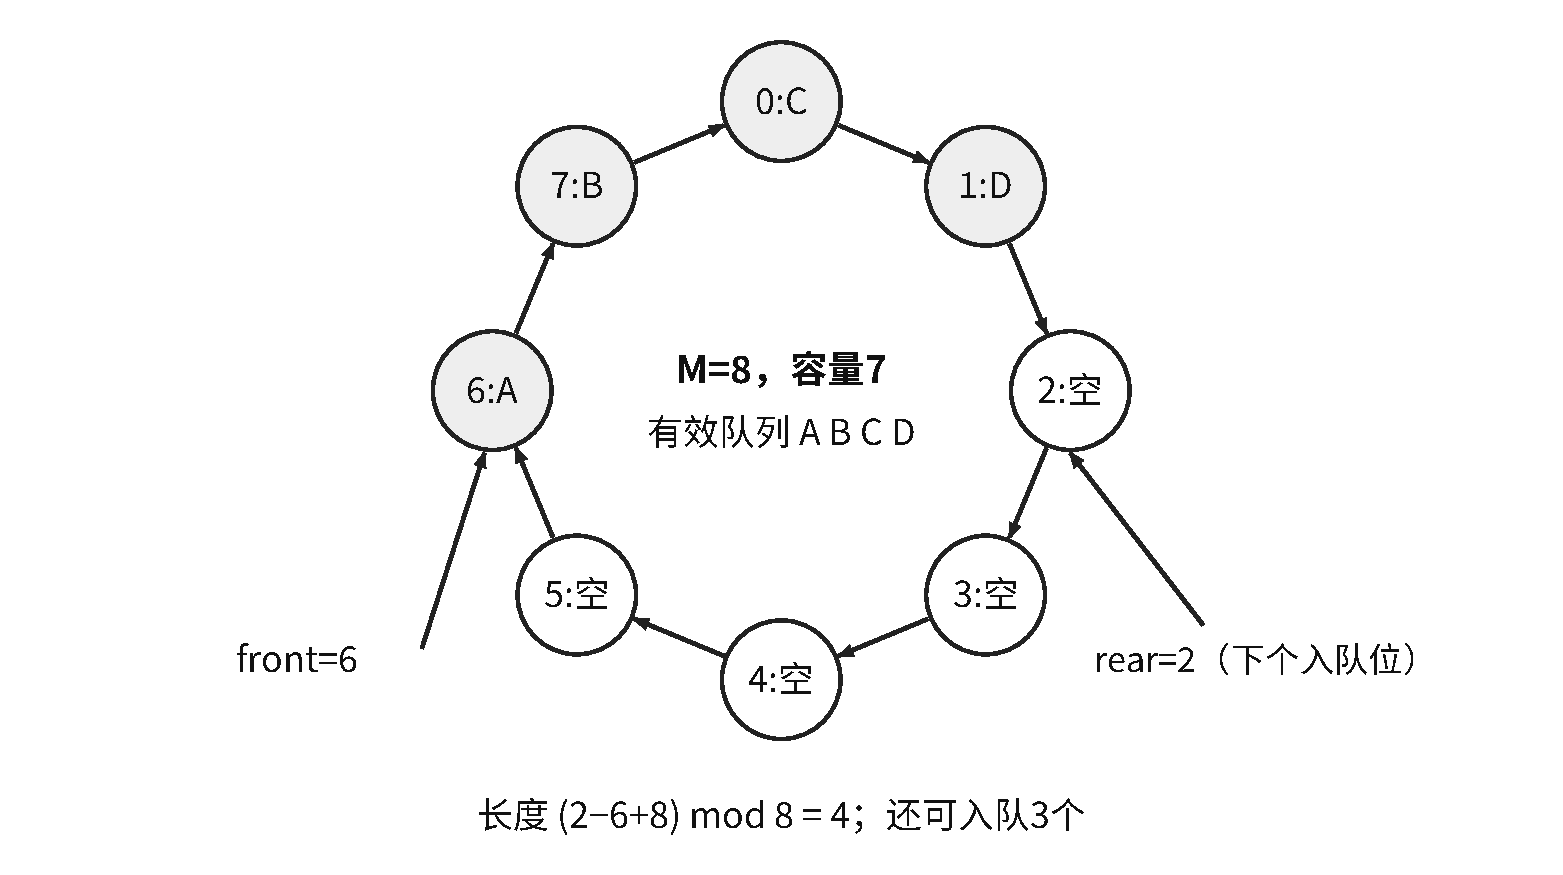
\includegraphics[width=\linewidth,height=125mm,keepaspectratio]{figures/DS_03_circular_queue.pdf}
\captionof{figure}{数组环绕时，下标大小不代表队列先后；本图采用牺牲一个单元}\label{ds-fig-circular}
\end{minipage}\par\medskip

若要求 \(M\) 个单元全部可用，可以增加 \texttt{size} 计数，或增加标志，区分最近一次使二者相等的是入队还是出队。此时``空''和``满''的判断依赖新增成员，不能仍照搬牺牲单元的满条件。

\subsection{例 3-2　换了 front 含义，长度公式是否改变}\label{DS03-ex2}

\begin{example}[配套例题]

〖3.2-006〗 循环队列存于数组 \texttt{A[\allowbreak{}21]\allowbreak{}}，\texttt{front} 指向队首元素的前一个位置，\texttt{rear} 指向队尾元素。当前 \texttt{front=\allowbreak{}8,\allowbreak{} rear=\allowbreak{}3}，队列长度为（　）。

A. 5　B. 6　C. 16　D. 17

\end{example}

\textbf{解析。} 有效元素从下标9开始，经过9至20，再经过0至3，共 \(12+4=16\) 个，答案为 \textbf{C}。公式仍可写成 \((3-8+21)\bmod21=16\)，是因为与前一约定相比，两个指针的含义都错开了一个位置。若只改变一个指针的含义，公式就未必不变。数组是 \texttt{A[\allowbreak{}0.\allowbreak{}.\allowbreak{}n]\allowbreak{}} 时实际有 \(n+1\) 个单元，取模也必须使用 \(n+1\)。

另一种常见表示令front仍指队头，而rear指当前队尾。可令初始front=0、rear=M\ensuremath{-}1；入队先推进rear再写入，出队先读取front再推进。牺牲一个单元时，空条件是\texttt{(\allowbreak{}rear+\allowbreak{}1)\allowbreak{}\%M=\allowbreak{}=\allowbreak{}front}，满条件是\texttt{(\allowbreak{}rear+\allowbreak{}2)\allowbreak{}\%M=\allowbreak{}=\allowbreak{}front}，长度为\texttt{(\allowbreak{}rear-front+\allowbreak{}1+\allowbreak{}M)\allowbreak{}\%M}。例如M=5、front=0、rear=3时有4个元素，已经满；front=0、rear=4则为空。它与本章正式SqQueue接口是不同表示，应连同初始化、动作次序和判空判满一起使用。

\section{链栈与链队列}\label{DS03-04}

链栈通常把链头作为栈顶，头插与头删都是 \(O(1)\)。动态分配可随数据量申请结点，因而通常不受预先给定的小容量数组限制；但入栈仍可能因可用内存不足而失败，出栈时也仍可能遇到空栈。

单链队列把链头作为队头，链尾作为队尾，并保存两个指针。若反过来从单链表尾部删除，必须找到尾结点的前驱，出队会变为 \(O(n)\)。带头结点的链队列空时 \texttt{front=\allowbreak{}=\allowbreak{}rear}，二者都指向头结点。入队时接到 \texttt{rear->\allowbreak{}next} 并更新 \texttt{rear}；出队时删除 \texttt{front->\allowbreak{}next}。

\par\medskip\noindent\begin{minipage}{\linewidth}
\BlueLines{2,6,8}
\begin{codeblock}[language={}]
dequeue(Q):
    if Q.front==Q.rear: return 失败
    p=Q.front->next
    x=p->data
    Q.front->next=p->next
    if Q.rear==p: Q.rear=Q.front
    释放 p
    return x
\end{codeblock}
\end{minipage}\par\medskip

最后一个数据结点出队时，必须让尾指针退回头结点；否则它指向已释放的空间。非空且不止一个元素时，无需改变尾指针，所以对``删除是否修改头尾指针''这类问题，答案取决于被删除的是否为最后一个元素。

只带队首指针的非循环双链表，要在另一端入队仍需找尾部；循环双链表则可通过 \texttt{front->\allowbreak{}prior} 直接取得尾部。比较结构时，应检查有没有可到达另一端的短链接，而不是看到``双链''就认定所有操作都为常数时间。

\section{多维数组的地址怎样计算}\label{DS03-05}

数组同一维度的下标取值范围固定，每个元素大小相同。设二维数组的行下标为 \(l_1\sim u_1\)，列下标为 \(l_2\sim u_2\)，列数 \(c=u_2-l_2+1\)，行数 \(r=u_1-l_1+1\)，每元素占 \(w\) 字节，首元素地址为 \(b\)。

按行优先时，在 \((i,j)\) 前有 \(i-l_1\) 个完整行及本行的 \(j-l_2\) 个元素，故

\[\operatorname{Addr}(A[i,j])=b+[(i-l_1)c+(j-l_2)]w.\]

按列优先时，先数完整列：

\[\operatorname{Addr}(A[i,j])=b+[(j-l_2)r+(i-l_1)]w.\]

例如 \texttt{A[\allowbreak{}2.\allowbreak{}.\allowbreak{}4]\allowbreak{}[\allowbreak{}−1.\allowbreak{}.\allowbreak{}2]\allowbreak{}} 按行优先存放，每元素4字节，\texttt{A[\allowbreak{}2]\allowbreak{}[\allowbreak{}−1]\allowbreak{}} 的地址为1000。\texttt{A[\allowbreak{}4]\allowbreak{}[\allowbreak{}1]\allowbreak{}} 前有 \(2\times4+2=10\) 个元素，字节地址为1040。下标差先得到``元素数''，最后乘元素宽度才得到字节偏移；按字编址的题则要统一成字地址再计算。

三维数组按行优先时，最右下标变化最快：\texttt{A[\allowbreak{}i]\allowbreak{}[\allowbreak{}j]\allowbreak{}[\allowbreak{}k]\allowbreak{}} 的相对元素位置为 \(((i-l_1)n_2+(j-l_2))n_3+(k-l_3)\)。可以逐维理解，不必另背一个没有下标原点的公式。

\section{对称、三角、三对角与稀疏矩阵}\label{DS03-06}

压缩存储利用元素间的确定关系，避免重复保存。\textbf{对称矩阵}满足 \(a_{ij}=a_{ji}\)，保存一侧三角即可；访问另一侧时交换 \(i,j\)。\textbf{三角矩阵}的三角区之外，元素全部相同，通常还要额外保存这个公共常量，它未必为0。\textbf{三对角矩阵}只在主对角线及相邻两条对角线上可能非零，共有 \(3n-2\) 个需要保存的位置。

下三角按行保存、原矩阵与数组下标均从0开始时，位置 \((i,j)\)（\(i\ge j\)）之前有 \(1+2+\cdots+i=i(i+1)/2\) 个元素，故数组下标为 \(i(i+1)/2+j\)。若原矩阵从1开始而数组从0开始，公式相应变成 \(i(i-1)/2+j-1\)。推导的顺序始终是``前面完整行或列数＋本行或列内偏移''。

\subsection{例 3-3　三对角矩阵的起止行不能一律算3个}\label{DS03-ex3}

\begin{example}[配套例题]

配套例题：100阶三对角矩阵 \(M\) 的元素 \(m_{i,j}\ (1\le i,j\le100)\) 按行优先依次压缩存入下标从0开始的一维数组 \(N\)。\(m_{30,30}\) 在 \(N\) 中的下标为（　）。

A. 86　B. 87　C. 88　D. 89

\end{example}

\textbf{解析。} 第一行有2个元素，第2至29行各有3个，共 \(2+28\times3=86\) 个在第30行之前。第30行依次保存 \(m_{30,29},m_{30,30},m_{30,31}\)，目标是本行第2个，因此下标为 \(86+1=87\)，答案为 \textbf{B}。这里87是从0开始的下标，目标是第88个被保存的元素。

\subsection{例 3-4　先用对称性换到实际保存的半边}\label{DS03-ex4}

\begin{example}[配套例题]

配套例题：10\ensuremath{\times}10对称矩阵 \(M\) 的上三角元素 \(m_{i,j}\ (1\le i\le j\le10)\) 按列优先存入 C 语言一维数组 \(N\)。\(m_{7,2}\) 在 \(N\) 中的下标为（　）。

A. 15　B. 16　C. 22　D. 23

\end{example}

\textbf{解析。} \(m_{7,2}=m_{2,7}\)，实际寻找第7列第2行。前6列各存 \(1,2,\ldots,6\) 个，共21个；本列目标前还有第1行1个元素，所以从0开始的下标为 \(21+1=22\)，答案为 \textbf{C}。不能先把下三角坐标直接代入上三角公式，再试图以加减1修正。

上三角若改为按行优先，各行长度为 \(n,n-1,\ldots,1\)；第 \(i\) 行之前有 \((i-1)(2n-i+2)/2\) 个保存位置。下三角若按列优先，各列长度同样递减，但列内偏移为 \(i-j\)。公式外形相近，决定它的是保存方向与下标原点。

\textbf{稀疏矩阵}的非零位置没有固定三角规律，需要连同位置一起保存。三元组顺序表记录 \texttt{(\allowbreak{}行,\allowbreak{}列,\allowbreak{}值)\allowbreak{}}，还须保存矩阵行列数与非零元数；十字链表为同一个非零元同时设置行链接和列链接。压缩后不能再按普通二维数组地址公式随机访问任意元素，查找与修改成本随表示方法而变。

\section{表达式、递归与层次处理}\label{DS03-07}

\subsection{括号与表达式中的``最近一个尚未完成对象''}\label{DS03-detail2}

左括号入栈；遇右括号时，栈顶必须是对应种类的左括号，匹配后弹出；扫描完后栈必须为空。\texttt{(\allowbreak{}[\allowbreak{})\allowbreak{}]\allowbreak{}} 中括号数量相等，但遇到第一个右圆括号时栈顶为左方括号，已经失败。这个过程正好需要最后遇到且尚未配对的对象，所以选择栈。

后缀表达式中，操作数先入栈，遇二元运算符时先弹出的数是\textbf{右操作数}，后弹出的是左操作数，计算后将结果入栈。减法、除法不能颠倒。合法的二元后缀表达式在遇到每个运算符时，栈中至少有两个可用值，最终恰好留下一个结果。

\subsection{例 3-5　弹出次序怎样影响减法}\label{DS03-ex5}

\begin{example}[配套例题]

配套例题：栈 \(S_1\) 保存整数，\(S_2\) 保存运算符。函数 F() 依次：（1）从 \(S_1\) 弹出操作数 a、b；（2）从 \(S_2\) 弹出运算符 op；（3）执行 b op a；（4）把结果压入 \(S_1\)。初始 \(S_1\) 自底向顶为5、8、3、2，\(S_2\) 自底向顶为 \texttt{*\allowbreak{}}、\texttt{−}、\texttt{+\allowbreak{}}。调用3次 F() 后，\(S_1\) 栈顶值是（　）。

A. \ensuremath{-}15　B. 15　C. \ensuremath{-}20　D. 20

\end{example}

\textbf{解析。} 第一次弹出2、3，用加法得到 \(3+2=5\)，整数栈变为5、8、5。第二次弹出5、8，用减法得到 \(8-5=3\)，栈变为5、3。第三次得到 \(5\times3=15\)，答案为 \textbf{B}。若第二次按弹出先后计算 \(5-8\)，就会得到错误的负数。

中缀转后缀可用运算符栈：操作数直接输出；左括号入栈；右括号触发输出直到匹配左括号；遇运算符时，先输出栈顶中优先级更高的运算符。对通常左结合的 \texttt{+\allowbreak{}、−、*\allowbreak{}、/\allowbreak{}}，同级也先弹出；若加入右结合运算符，同优先级的处理规则需要调整。

例如 \(x+y(z-u)/v\)（其中相邻表示乘法）先把括号内写成 \texttt{zu−}，乘除按左结合形成 \texttt{yzu−*\allowbreak{}v/\allowbreak{}}，最后与 x 相加，得 \texttt{xyzu−*\allowbreak{}v/\allowbreak{}+\allowbreak{}}。这里的输出顺序表达运算依赖，而不是把原式的符号按种类重新排列。

\subsection{递归返回前保存了什么}\label{DS03-detail3}

递归调用栈保存尚未完成的调用。调用树的一个结点表示一次调用，不能把函数返回值当作调用次数。对于

\par\medskip\noindent\begin{minipage}{\linewidth}
\BlueLines{2,3}
\begin{codeblock}[language=C]
int F(int n) {
    if (n<=3) return 1;
    return F(n-2)+F(n-4)+1;
}
\end{codeblock}
\end{minipage}\par\medskip

令 \(C(n)\) 表示含当前调用在内的调用次数，则 \(n\le3\) 时 \(C(n)=1\)，否则 \(C(n)=1+C(n-2)+C(n-4)\)。因此 \(C(4)=C(2)+C(0)+1=3\)，\(C(6)=1+3+1=5\)，\(C(8)=1+5+3=9\)。式中返回值的``＋1''不是另一次函数调用；次数递推中的``＋1''是当前调用本身。此过程对应〖3.3-006〗的递归调用模型。

C/C++ 对加号两侧函数调用的求值先后并不一概保证从左到右。若题目问``第几个被调用''，应检查答案是否依赖这个先后，不能把一种习惯顺序当作语言保证。调用总数与最终结果在本例不受这个先后影响。另如〖3.3-007〗把递归式改为 \texttt{func(\allowbreak{}x-2)\allowbreak{}+\allowbreak{}func(\allowbreak{}x-4)\allowbreak{}}、基例返回2，并计算 \texttt{func(\allowbreak{}func(\allowbreak{}5)\allowbreak{})\allowbreak{}}：必须先完成内层func(5)，它和func(3)、func(1)共3次调用，结果为4，所以第4次是外层func(4)；内层两个基例谁先执行不影响这个结论。

层次处理需要先进先出的队列：先发现的一层结点必须先扩展，后发现的下一层排在后面。第5章层序遍历与第6章 BFS 都用这条约束，但图还需 \texttt{visited} 防止同一顶点反复入队。

\subsection{阶乘、Fibonacci与重复子问题}\label{DS03-recursion-model}

下面两段保留课件的递归定义。输入n为非负整数，计算结果须在int可表示范围内。

\par\medskip\noindent\begin{minipage}{\linewidth}
\BlueLines{2,3,6}
\begin{codeblock}[language=C]
int factorial(int n) {
    if (n == 0 || n == 1) return 1;
    else return n * factorial(n - 1);
}
int Fib(int n) {
    if (n == 0) return 0;
    else if (n == 1) return 1;
    else return Fib(n - 1) + Fib(n - 2);
}
\end{codeblock}
\end{minipage}\par\medskip

factorial(10)沿10、9、\ldots、1依次深入，最多同时保留10层调用，随后按相反次序返回并完成乘法。Fib(4)的调用树有9个结点，返回值为3，最长未返回调用链却只有4层；Fib(2)重复出现两次。朴素Fib递归的时间满足\(T(n)=T(n-1)+T(n-2)+O(1)\)，呈指数增长，递归工作栈为\(O(n)\)。每层传递两个递归分支，不意味着空间也按整棵调用树相加；一个分支返回后，其空间可供另一个使用。保存已算子问题或改用迭代可减少重复计算，改变算法后须重新分析代价。

\par\medskip\noindent\begin{minipage}{\linewidth}
\centering
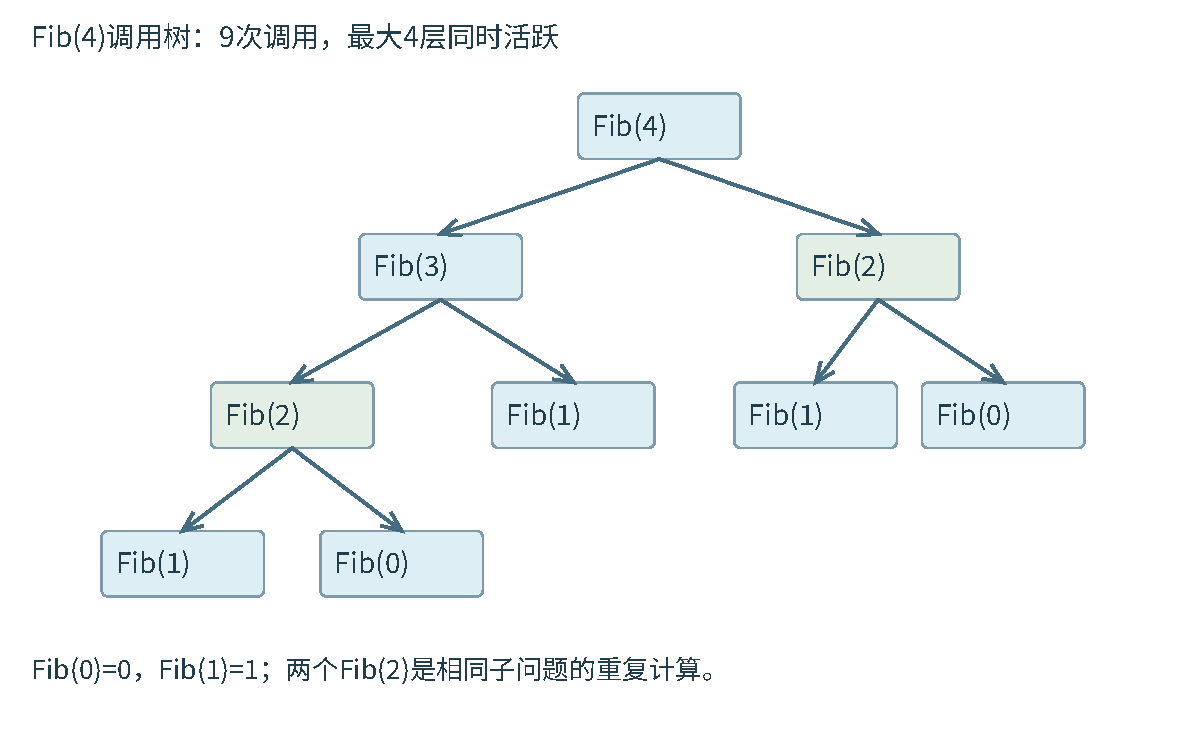
\includegraphics[width=\linewidth,height=125mm,keepaspectratio]{figures/DS03_fib_tree.pdf}
\captionof{figure}{Fib(4)的完整调用树：重复子问题与最大同时活跃调用链}\label{ds03-fig-fib}
\end{minipage}\par\medskip

\section{栈与队列的教材接口}\label{DS03-code}

\begin{definition}[先约定指针指向什么，再写边界]

顺序栈中的top可以指栈顶元素，也可以指下一空位；循环队列中的front/rear也有不同语义。表示约定决定空满条件、增减时机和长度公式。同一个变量名并不保证同一种表示，改题时先画空状态和单元素状态。

\end{definition}

下面采用教材的\texttt{SqStack}，\texttt{top}指当前栈顶；下标从0开始，空栈\texttt{top=\allowbreak{}-1}。\texttt{ElemType}按具体应用定义为元素类型，下面可取整型。

\par\medskip\noindent\begin{minipage}{\linewidth}
\BlueLines{8,10,12}
\begin{codeblock}[language=C++]
#define MaxSize 100
typedef int ElemType;
typedef struct {
    ElemType data[MaxSize];
    int top;
} SqStack;
void InitStack(SqStack &S) { S.top = -1; }
bool StackEmpty(SqStack S) { return S.top == -1; }
bool Push(SqStack &S, ElemType x) {
    if (S.top == MaxSize - 1) return false;
    S.data[++S.top] = x;
    return true;
}
bool Pop(SqStack &S, ElemType &x) {
    if (S.top == -1) return false;
    x = S.data[S.top--];
    return true;
}
bool GetTop(SqStack S, ElemType &x) {
    if (S.top == -1) return false;
    x = S.data[S.top];
    return true;
}
\end{codeblock}
\end{minipage}\par\medskip

读栈顶不改变top，出栈才将top减1。若栈顶指向下一空位，压入顺序应为\texttt{data[\allowbreak{}top+\allowbreak{}+\allowbreak{}]\allowbreak{}=\allowbreak{}x}，弹出则为\texttt{x=\allowbreak{}data[\allowbreak{}--top]\allowbreak{}}；这是一套独立表示，不能只改初始化而保留其余操作。

循环队列使用教材的\texttt{SqQueue}，front指队头元素、rear指下一入队位置，牺牲一个单元。

\par\medskip\noindent\begin{minipage}{\linewidth}
\BlueLines{6,8,11}
\begin{codeblock}[language=C++]
typedef struct {
    ElemType data[MaxSize];
    int front, rear;
} SqQueue;
void InitQueue(SqQueue &Q) { Q.front = Q.rear = 0; }
bool QueueEmpty(SqQueue Q) { return Q.front == Q.rear; }
bool EnQueue(SqQueue &Q, ElemType x) {
    if ((Q.rear + 1) % MaxSize == Q.front) return false;
    Q.data[Q.rear] = x;
    Q.rear = (Q.rear + 1) % MaxSize;
    return true;
}
bool DeQueue(SqQueue &Q, ElemType &x) {
    if (Q.front == Q.rear) return false;
    x = Q.data[Q.front];
    Q.front = (Q.front + 1) % MaxSize;
    return true;
}
bool GetHead(SqQueue Q, ElemType &x) {
    if (Q.front == Q.rear) return false;
    x = Q.data[Q.front];
    return true;
}
\end{codeblock}
\end{minipage}\par\medskip

入队先写rear位置再推进rear，出队先取front位置再推进front。空满检查均在修改之前进行，失败操作保持原状态，输出参数也不赋新值。读队头只读取，不出队。

\begin{proof}[环形长度公式来自有向距离]

从front沿数组下标递增方向走到rear，步数就是有效元素数。未绕回时为rear\ensuremath{-}front，绕回时为M\ensuremath{-}front+rear，合并为\((rear-front+M)\bmod M\)。牺牲一个单元将步数限制在0至M\ensuremath{-}1，从而只让0表示空；若允许M个元素，模运算会把长度M也变成0，必须增加size或标志保存这一个区别。

\end{proof}

\begin{wideblock}

\par\medskip\noindent\begin{minipage}{\linewidth}\fontsize{9.3}{12}\selectfont\begin{tabularx}{\linewidth}{@{}YYYY@{}}
\toprule\noalign{}
环形队列策略 & 空条件 & 满条件 & 可用容量 \\
\midrule\noalign{}


牺牲一个单元 & front=rear & (rear+1) mod M=front & M\ensuremath{-}1 \\
增加size计数 & size=0 & size=M & M \\
增加最近操作tag & front=rear且tag为出队 & front=rear且tag为入队 & M \\
\bottomrule\end{tabularx}
\end{minipage}\par\medskip

\end{wideblock}

tag方案初始设为``出队''态，初始化即表示空；成功入队/出队后更新tag。计数方案每次成功修改长度，失败操作不能改size。链队列没有预设数组容量，但申请新结点仍可能失败，不能将``不判数组满''理解为内存无限。

\section{矩阵压缩：由坐标到下标，再从下标恢复坐标}\label{DS03-matrix-method}

\begin{methodbox}[完整行数加行内偏移]

每次先写清：矩阵坐标从0还是1开始、压缩数组从0还是1开始、上/下三角、行/列优先。若是对称矩阵，先把目标换到实际保存的半边。最后数前面完整行或列，再加本行/列内偏移；不要用最后加减1修补错误的保存方向。

\end{methodbox}

对于坐标从0开始、按行保存下三角的矩阵，令\(T_i=i(i+1)/2\)，则\(k=T_i+j\)。反向给定有效数组下标k时，先找到唯一满足\(T_i\le k<T_{i+1}\)的i，再令\(j=k-T_i\)。数学上

\[i=\left\lfloor\frac{\sqrt{8k+1}-1}{2}\right\rfloor,\qquad j=k-\frac{i(i+1)}2.\]

例如k=8，因\(T_3=6\le8<T_4=10\)，得\(i=3,j=2\)。实现时若用浮点平方根，应以整数三角数边界复核，防止舍入把边界分到相邻行。

坐标从1开始、压缩数组从0开始时，上三角行优先下标为

\[k=\frac{(i-1)(2n-i+2)}2+(j-i),\quad1\le i\le j\le n.\]

下三角列优先则为

\[k=\frac{(j-1)(2n-j+2)}2+(i-j),\quad1\le j\le i\le n.\]

三角矩阵的公共常量区可另存一个值，所需空间为\(n(n+1)/2+1\)；对称矩阵只保存一侧即可，不需要这个公共常量单元。三对角矩阵\(n\ge2\)时按行存3n\ensuremath{-}2个有效位置，坐标从1、数组从0的统一公式为\(k=2i+j-3\)，前提是\(|i-j|\le1\)且坐标不越界。n=1时只有一个元素，应按单元素矩阵处理，不再套首尾行各2个的解释。

稀疏矩阵中零元位置不具有固定三角规律。三元组的``下标''表示第几个非零记录，不能直接由坐标用普通二维地址公式得到；修改原来的零元为非零元时，可能需要插入记录并调整次序或链接。

\section{典型应用的失败条件}\label{DS03-app-method}

中缀表达式将运算符写在左右操作数之间；前缀写在两者之前，后缀写在两者之后。前缀求值从右向左扫描，遇运算符先弹出的值是左操作数、后弹出的值是右操作数；后缀从左向右扫描则先弹出右操作数。方向与角色要一起记。

例如\(x+y(z-u)/v\)按通常左结合规则，前缀为\texttt{+\allowbreak{} x /\allowbreak{} *\allowbreak{} y - z u v}，后缀为\texttt{x y z u - *\allowbreak{} v /\allowbreak{} +\allowbreak{}}。两种形式都用位置表达运算依赖而省去括号；不是简单地把所有运算符搬到字符串开头或末尾。

\begin{methodbox}[按尚未完成对象的次序选结构]

最近进入且尚未结束的对象要先处理，用栈：括号配对、函数调用、表达式中等待右操作数的运算。最早进入且尚未服务的对象先处理，用队列：层序遍历、BFS、先来先服务。操作系统的就绪队列只是管理等待对象，实际调度策略未必总是FIFO。

\end{methodbox}

后缀表达式求值必须同时检查：遇二元运算符时至少有两个操作数、除数合法、扫描末尾恰好留下一个结果。仅仅``最终留下一个数''不足以排除中途栈下溢。例如\texttt{1 +\allowbreak{} 2}按后缀语法扫描，在加号处就没有两个数；\texttt{1 2 3 +\allowbreak{}}则扫描后还剩两个值。

\begin{example}[自拟：括号数量正确仍可失败]

输入\texttt{(\allowbreak{}[\allowbreak{})\allowbreak{}]\allowbreak{}}中左右圆括号和左右方括号数量分别相等。用栈检查时，在哪一个字符首次失败？

\end{example}

前两个字符依次入栈，栈顶为\texttt{[\allowbreak{}}；读到第三个字符\texttt{)\allowbreak{}}时，它要求栈顶为\texttt{(\allowbreak{}}，因此立即失败。只统计每类括号数量看不到嵌套关系，错误发生在第三个字符，不能等扫描完再随意重新配对。

\section{链栈、链队列与共享栈的实现边界}\label{DS03-linked-code}

链栈通常不带头结点，Ltop指向当前栈顶，空栈为NULL。以下采用教材的链栈结点定义，申请与释放使用malloc/free。

\par\medskip\noindent\begin{minipage}{\linewidth}
\BlueLines{7,11,14}
\begin{codeblock}[language=C++]
typedef struct Linknode {
    ElemType data;
    struct Linknode *next;
} *LiStack;
bool Push(LiStack &S, ElemType x) {
    LiStack p = (LiStack)malloc(sizeof(struct Linknode));
    if (p == NULL) return false;
    p->data = x;
    p->next = S;
    S = p;
    return true;
}
bool Pop(LiStack &S, ElemType &x) {
    if (S == NULL) return false;
    LiStack p = S;
    x = p->data;
    S = p->next;
    free(p);
    return true;
}
\end{codeblock}
\end{minipage}\par\medskip

链栈从链头入栈、出栈，均为\(O(1)\)；若改在普通单链表尾部出栈，定位尾结点前驱会变为线性时间。初始化令S为空即可；销毁时重复弹出或逐结点释放。

\subsection{带头结点链队列}\label{DS03-linkqueue-code}

头结点使空队列和一般出队的前驱统一。front始终指头结点，rear指最后一个结点；空时二者指向同一个头结点。

\par\medskip\noindent\begin{minipage}{\linewidth}
\BlueLines{12,21,25}
\begin{codeblock}[language=C++]
typedef struct LinkNode {
    ElemType data;
    struct LinkNode *next;
} LinkNode;
typedef struct {
    LinkNode *front, *rear;
} LinkQueue;
void InitQueue(LinkQueue &Q) {
    Q.front = Q.rear = (LinkNode *)malloc(sizeof(LinkNode));
    Q.front->next = NULL;
}
bool IsEmpty(LinkQueue Q) { return Q.front == Q.rear; }
void EnQueue(LinkQueue &Q, ElemType x) {
    LinkNode *s = (LinkNode *)malloc(sizeof(LinkNode));
    s->data = x;
    s->next = NULL;
    Q.rear->next = s;
    Q.rear = s;
}
bool DeQueue(LinkQueue &Q, ElemType &x) {
    if (Q.front == Q.rear) return false;
    LinkNode *p = Q.front->next;
    x = p->data;
    Q.front->next = p->next;
    if (Q.rear == p) Q.rear = Q.front;
    free(p);
    return true;
}
\end{codeblock}
\end{minipage}\par\medskip

初始化和入队保留王道课件的void接口，以内存申请成功为前提。实际程序须检查malloc结果，并在申请失败时保持原队列。最后一个数据结点出队后，必须把rear退回front；随后再次入队才有有效尾指针。销毁链队列还需释放头结点。

\par\medskip\noindent\begin{minipage}{\linewidth}
\centering
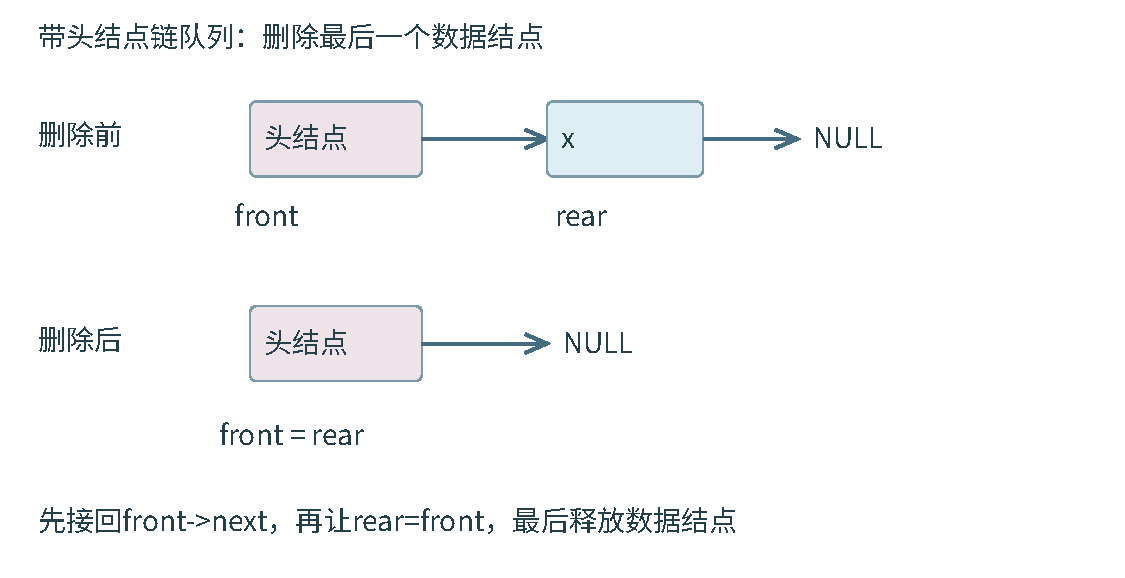
\includegraphics[width=\linewidth,height=125mm,keepaspectratio]{figures/DS03_linkqueue_last.pdf}
\captionof{figure}{最后一个数据结点出队后，front与rear共同指向有效头结点}\label{ds03-fig-linkqueue}
\end{minipage}\par\medskip

若采用不带头结点的版本，首次入队须同时建立front和rear，最后一次出队须同时置空二者。

以下是另一套独立实现，仍使用LinkQueue类型，但front指首个数据结点。不能与前面的带头结点接口混合调用。

\par\medskip\noindent\begin{minipage}{\linewidth}
\BlueLines{4,9,17}
\begin{codeblock}[language=C++]
void InitQueue(LinkQueue &Q) {
    Q.front = Q.rear = NULL;
}
bool IsEmpty(LinkQueue Q) { return Q.front == NULL; }
void EnQueue(LinkQueue &Q, ElemType x) {
    LinkNode *s = (LinkNode *)malloc(sizeof(LinkNode));
    s->data = x;
    s->next = NULL;
    if (Q.front == NULL)
        Q.front = Q.rear = s;
    else {
        Q.rear->next = s;
        Q.rear = s;
    }
}
bool DeQueue(LinkQueue &Q, ElemType &x) {
    if (Q.front == NULL) return false;
    LinkNode *p = Q.front;
    x = p->data;
    Q.front = p->next;
    if (Q.rear == p) Q.rear = NULL;
    free(p);
    return true;
}
\end{codeblock}
\end{minipage}\par\medskip

\subsection{共享栈的容量如何协同}\label{DS03-share-code}

\par\medskip\noindent\begin{minipage}{\linewidth}
\begin{codeblock}[language=C++]
typedef struct {
    ElemType data[MaxSize];
    int top0, top1;
} ShStack;
void InitStack(ShStack &S) {
    S.top0 = -1;
    S.top1 = MaxSize;
}
\end{codeblock}
\end{minipage}\par\medskip

教材\texttt{ShStack}的两端栈顶初值为\texttt{top0=\allowbreak{}-1,\allowbreak{}top1=\allowbreak{}MaxSize}，共享空闲区在两栈顶之间，满条件\texttt{top1-top0=\allowbreak{}=\allowbreak{}1}。若入0号栈，先检查满，再令\texttt{data[\allowbreak{}+\allowbreak{}+\allowbreak{}top0]\allowbreak{}=\allowbreak{}x}；入1号栈则令\texttt{data[\allowbreak{}--top1]\allowbreak{}=\allowbreak{}x}。出0号栈取\texttt{data[\allowbreak{}top0--]\allowbreak{}}，出1号栈取\texttt{data[\allowbreak{}top1+\allowbreak{}+\allowbreak{}]\allowbreak{}}，各自先判空。

共享只提高同一块空间的利用率；两个栈仍各自满足后进先出。若一栈已占满全部单元，另一栈即使为空也不能继续入栈。

\section{括号匹配的完整状态检查}\label{DS03-bracket-code}

用字符作为ElemType，复用顺序栈接口。新左括号意味着最近一个尚未完成对象；右括号必须关闭栈顶的同种左括号。

\par\medskip\noindent\begin{minipage}{\linewidth}
\BlueLines{6,7,8}
\begin{codeblock}[language=C++]
bool bracketCheck(char str[], int length) {
    SqStack S;
    InitStack(S);
    for (int i = 0; i < length; ++i) {
        char c = str[i];
        if (c == '(' || c == '[' || c == '{') {
            if (!Push(S, c)) return false;
        } else if (c == ')' || c == ']' || c == '}') {
            ElemType x;
            if (!Pop(S, x)) return false;
            if ((c == ')' && x != '(') ||
                (c == ']' && x != '[') ||
                (c == '}' && x != '{')) return false;
        }
    }
    return StackEmpty(S);
}
\end{codeblock}
\end{minipage}\par\medskip

遇右括号但栈为空，属于右括号过早；栈顶类型不符，属于交叉嵌套；扫描结束栈非空，属于左括号尚未关闭。每字符只处理常数次，时间\(O(n)\)，最坏保留n个左括号，辅助空间\(O(n)\)；定长栈实现还要求实际所需深度不超过容量。

\section{按课件表达式保留完整转换过程}\label{DS03-expression-trace}

中缀表达式\texttt{A+\allowbreak{}B-C*\allowbreak{}D/\allowbreak{}E+\allowbreak{}F}的运算次序为：先A+B，再C*D，再除以E，再从A+B减去该商，最后加F。按左结合规则得到后缀：

\par\medskip\noindent\begin{minipage}{\linewidth}
\begin{codeblock}[language={}]
A B + C D * E / - F +
\end{codeblock}
\end{minipage}\par\medskip

\par\medskip\noindent\begin{minipage}{\linewidth}\fontsize{9.3}{12}\selectfont\begin{tabularx}{\linewidth}{@{}YYY@{}}
\toprule\noalign{}
当前符号 & 运算符栈（底到顶） & 已输出后缀 \\
\midrule\noalign{}


A & 空 & A \\
+、B & + & A B \\
\ensuremath{-} & \ensuremath{-} & A B + \\
C、*、D & \ensuremath{-}、* & A B + C D \\
/ & \ensuremath{-}、/ & A B + C D * \\
E & \ensuremath{-}、/ & A B + C D * E \\
+ & + & A B + C D * E / \ensuremath{-} \\
\bottomrule\end{tabularx}
\end{minipage}\par\medskip

\par\medskip\noindent\begin{minipage}{\linewidth}\fontsize{9.3}{12}\selectfont\begin{tabularx}{\linewidth}{@{}YYY@{}}
\toprule\noalign{}
当前符号 & 运算符栈（底到顶） & 已输出后缀 \\
\midrule\noalign{}


F、扫描结束 & 空 & A B + C D * E / \ensuremath{-} F + \\
\bottomrule\end{tabularx}
\end{minipage}\par\medskip

遇到\texttt{/\allowbreak{}}时先弹同级\texttt{*\allowbreak{}}，对应乘除左结合；遇到最后一个\texttt{+\allowbreak{}}时，先弹除号再弹减号。对于\texttt{A+\allowbreak{}B*\allowbreak{}(\allowbreak{}C-D)\allowbreak{}-E/\allowbreak{}F}，括号内的减法先完成，得到\texttt{A B C D - *\allowbreak{} +\allowbreak{} E F /\allowbreak{} -}。左括号只作为界限保存在栈中，不进入后缀输出。

课件的数值表达式

\[((15/(7-(1+1)))\times3)-(2+(1+1))\]

对应后缀为\texttt{15 7 1 1 +\allowbreak{} - /\allowbreak{} 3 *\allowbreak{} 2 1 1 +\allowbreak{} +\allowbreak{} -}。依次计算\(1+1=2\)、\(7-2=5\)、\(15/5=3\)、\(3\times3=9\)，右部分为\(2+(1+1)=4\)，结果为5。数字15是一个操作数，不能按字符1和5分开入栈。模拟可知操作数栈峰值为4个值，这和表达式的字符总数不同。

前缀形式用``运算符、左操作数、右操作数''表达同一依赖。从右向左求前缀值时，先弹出的数为左操作数；从左向右求后缀值时，先弹出的数为右操作数。把两种扫描方向混用，会在减除法中得到错误结果。

\subsection{直接用两个栈计算中缀表达式}\label{DS03-infix-eval}

也可以将``中缀转后缀''与``后缀求值''融合：操作数立即压入操作数栈；运算符和括号按转换算法管理。每当转换规则本应输出一个运算符时，直接从操作数栈先弹右操作数、再弹左操作数，计算后将结果压回。左括号仍只作边界，不参与运算；表达式结束时清理运算符栈。

以\texttt{A+\allowbreak{}B-C*\allowbreak{}D/\allowbreak{}E+\allowbreak{}F}为例，在读到减号时，先弹出加号并把A+B压回；读到除号时，先完成C\emph{D；读到最后一个加号时，依次完成(C}D)/E和(A+B)\ensuremath{-}(C*D)/E；最后再加F。这与后缀\texttt{A B +\allowbreak{} C D *\allowbreak{} E /\allowbreak{} - F +\allowbreak{}}表达同一依赖。两个栈分别保存``尚未归约的操作数''和``尚未确定何时执行的运算符''，不可把运算符与值混放在同一种栈元素模型中。

除括号配对外，还应检查操作数数量、运算符合法性、除零及最终结果数；若题目包含一元负号或多位数，应先按词法单元识别，再应用相应操作数个数的规则。

\section{数组与特殊矩阵的定位总表}\label{DS03-matrix-table}

下表统一规定：原矩阵坐标从1开始，压缩数组B下标从0开始；n为阶数。先依据对称性换到实际保存的三角区，再计算k。

\begin{wideblock}

\par\medskip\noindent\begin{minipage}{\linewidth}\fontsize{9.3}{12}\selectfont\begin{tabularx}{\linewidth}{@{}YYY@{}}
\toprule\noalign{}
保存区域与次序 & 合法坐标 & 压缩下标k \\
\midrule\noalign{}


下三角行优先 & \(i\ge j\) & \(i(i-1)/2+j-1\) \\
上三角列优先 & \(i\le j\) & \(j(j-1)/2+i-1\) \\
上三角行优先 & \(i\le j\) & \((i-1)(2n-i+2)/2+j-i\) \\
下三角列优先 & \(i\ge j\) & \((j-1)(2n-j+2)/2+i-j\) \\
三对角行优先 & \(|i-j|\le1\) & \(2i+j-3\) \\
\bottomrule\end{tabularx}
\end{minipage}\par\medskip

\end{wideblock}

对称矩阵保存\(n(n+1)/2\)个元素即可。三角矩阵另一个区域是同一个公共常量，需再保存一个常量单元，共\(n(n+1)/2+1\)个；公共常量不必为0。三对角矩阵n\ensuremath{\ge}2时保存\(3n-2\)个元素，首尾行各2个，中间每行3个。n=1时只有一个有效位置，应直接按单元素处理。

\par\medskip\noindent\begin{minipage}{\linewidth}
\centering
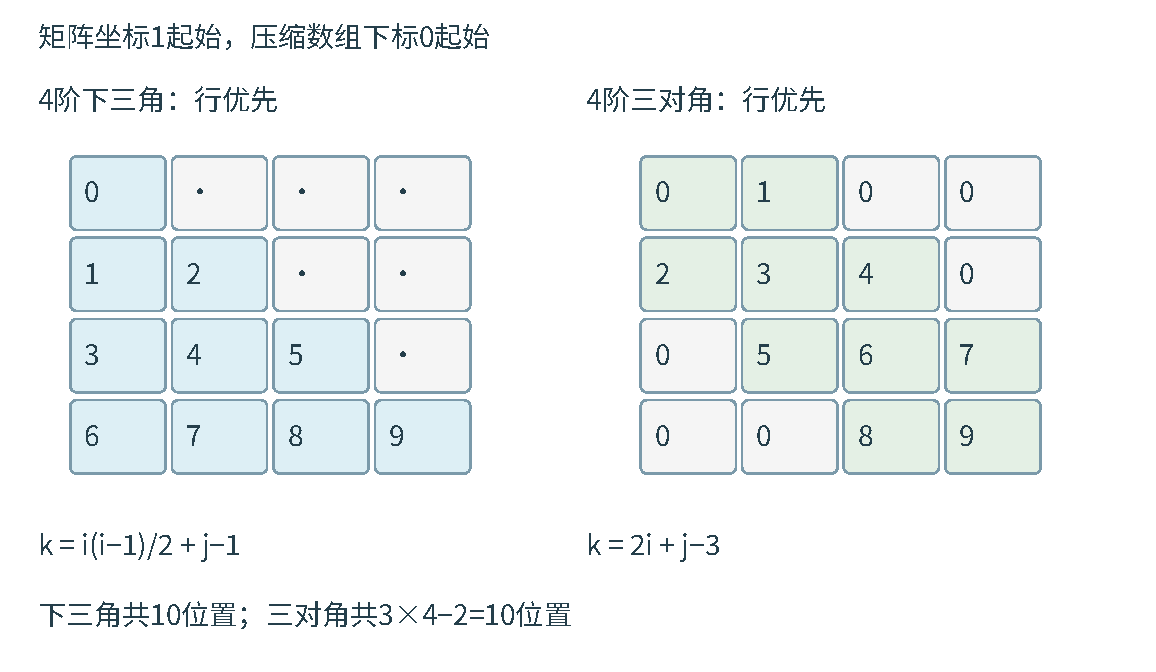
\includegraphics[width=\linewidth,height=125mm,keepaspectratio]{figures/DS03_matrix_positions.pdf}
\captionof{figure}{4阶下三角与三对角矩阵的压缩位置，矩阵1起始、数组0起始}\label{ds03-fig-matrix}
\end{minipage}\par\medskip

反向给定三对角压缩下标k时，第i行之前有\(3(i-1)-1\)个保存位置（首行单独核对），第i行结束前共\(3i-1\)个。因此可以取

\[i=\left\lceil\frac{k+2}{3}\right\rceil,\qquad j=k-2i+3.\]

行号也可写为\(i=\lfloor(k+1)/3\rfloor+1\)，与上述向上取整形式等价；应先确定i再求j。

例如k=87，\(i=\lceil89/3\rceil=30\)，\(j=87-60+3=30\)，与例3-3一致。前提是\(0\le k<3n-2\)且n\ensuremath{\ge}2；得到坐标后还可复核\(|i-j|\le1\)。

课件的5行6列稀疏矩阵有六个非零项，按行次序的三元组为：

\par\medskip\noindent\begin{minipage}{\linewidth}\fontsize{9.3}{12}\selectfont\begin{tabularx}{\linewidth}{@{}YYY@{}}
\toprule\noalign{}
行i & 列j & 值v \\
\midrule\noalign{}


1 & 3 & 4 \\
1 & 6 & 5 \\
2 & 2 & 3 \\
2 & 4 & 9 \\
3 & 5 & 7 \\
4 & 2 & 2 \\
\bottomrule\end{tabularx}
\end{minipage}\par\medskip

第5行全零，仍属于矩阵；只看非零记录无法恢复总行数，所以三元组表还要记录矩阵总行数、总列数和非零元数。十字链表中同一个非零结点同时进入行链和列链，修改时须维护两套联系。稀疏仅说明非零元少，不能据此使用三角矩阵的固定位置公式。

\section{主动回忆自测}\label{DS03-check}

第2题引自王道书，其余为原创补充，检查表示约定。

\begin{enumerate}
\def\labelenumi{\arabic{enumi}.}
\tightlist
\item
  数组有8个单元、牺牲一个单元的循环队列，\texttt{front=\allowbreak{}6,\allowbreak{}rear=\allowbreak{}2}，长度是多少？还能再入队几个元素？
\item
  〖3.1-025〗顺序共享栈 \texttt{Share[\allowbreak{}0.\allowbreak{}.\allowbreak{}n−1]\allowbreak{}}，第一个栈顶top1初值\ensuremath{-}1，第二个栈顶top2初值n，栈满条件是（　）。A. \texttt{top2−top1=\allowbreak{}=\allowbreak{}1}　B. \texttt{top1−top2=\allowbreak{}=\allowbreak{}1}　C. \texttt{top1=\allowbreak{}=\allowbreak{}top2}　D. 都不对
\item
  下标从1开始的三对角矩阵，若压缩数组也从1开始，非边界行元素 \(a_{i,j}\) 的位置如何计算？
\end{enumerate}

\textbf{答案。} 1. 长度 \((2-6+8)\bmod8=4\)，最大容量7，还能入队3个。2. \textbf{A}，两栈顶相邻时已无可用单元，不能等栈顶重合才判满。3. 前面有 \(2+3(i-2)=3i-4\) 个元素，本行从 \(j=i-1\) 开始，故从1开始的位置为 \(3i-4+[j-(i-1)]+1=2i+j-2\)；前提为 \(2\le i\le n-1\) 且 \(|i-j|\le1\)，首尾行须按实际保存位置解释。

\subsection{补充自拟回忆题}\label{DS03-recall-extra}

\begin{recallcard}[先画状态，再作判断]

\begin{enumerate}
\def\labelenumi{\arabic{enumi}.}
\setcounter{enumi}{3}
\tightlist
\item
  入栈顺序为a、b、c，输出c、a、b是否合法？第一次失败时栈顶是谁？
\item
  带头结点链队列删除最后一个数据结点时，front和rear应指向哪里？
\item
  同一个n阶对称矩阵，为什么下三角行优先和上三角列优先有相同的三角数结构？坐标如何转换？
\item
  后缀表达式\texttt{8 3 - 2 /\allowbreak{}}的值是多少？若按整数除法计算，先弹出的数是什么角色？
\item
  递归访问n个结点，最大同时活跃调用数一定为n吗？应由哪个结构参数决定？
\end{enumerate}

\end{recallcard}

\begin{solution}[补充题核对答案]

\begin{enumerate}
\def\labelenumi{\arabic{enumi}.}
\setcounter{enumi}{3}
\tightlist
\item
  不合法。弹出c后栈中为a、b，想输出a时栈顶是b，而输入已用尽。
\item
  front仍指有效头结点，rear必须退回front；头结点的next为空。rear不能留在已释放的数据结点上。
\item
  一边各行保存1、2、\ensuremath{\cdots}个元素，另一边各列也保存1、2、\ensuremath{\cdots}个。先用aij=aji交换坐标，再按对应行或列求偏移。
\item
  先计算8\ensuremath{-}3=5，再作5/2，整数结果为2；每次先弹出右操作数，除法的除数是先弹出的2。
\item
  不一定。由最长未返回调用链决定；树遍历通常取树高h，最坏链形树才可达到n。
\end{enumerate}

\end{solution}
